%%
%% This is file `sample-sigconf.tex',
%% generated with the docstrip utility.
%%
%% The original source files were:
%%
%% samples.dtx  (with options: `all,proceedings,bibtex,sigconf')
%% 
%% IMPORTANT NOTICE:
%% 
%% For the copyright see the source file.
%% 
%% Any modified versions of this file must be renamed
%% with new filenames distinct from sample-sigconf.tex.
%% 
%% For distribution of the original source see the terms
%% for copying and modification in the file samples.dtx.
%% 
%% This generated file may be distributed as long as the
%% original source files, as listed above, are part of the
%% same distribution. (The sources need not necessarily be
%% in the same archive or directory.)
%%
%%
%% Commands for TeXCount
%TC:macro \cite [option:text,text]
%TC:macro \citep [option:text,text]
%TC:macro \citet [option:text,text]
%TC:envir table 0 1
%TC:envir table* 0 1
%TC:envir tabular [ignore] word
%TC:envir displaymath 0 word
%TC:envir math 0 word
%TC:envir comment 0 0
%%
%% The first command in your LaTeX source must be the \documentclass
%% command.
%%
%% For submission and review of your manuscript please change the
%% command to \documentclass[manuscript, screen, review]{acmart}.
%%
%% When submitting camera ready or to TAPS, please change the command
%% to \documentclass[sigconf]{acmart} or whichever template is required
%% for your publication.
%%
%%
\documentclass[sigconf]{acmart}
%%



%% \BibTeX command to typeset BibTeX logo in the docs
\usepackage{subcaption}
\usepackage{float}

%use placeins with float barrier to fix position of fig 4a 4b 4c 4d
\usepackage{placeins}

%use labelfont, labelsep for removing ":" to fix caption of 4a 4b 4c 4d
\usepackage[labelfont=bf,labelsep=none]{caption}

\AtBeginDocument{%
  \providecommand\BibTeX{{%
    Bib\TeX}}}

%% Rights management information.  This information is sent to you
%% when you complete the rights form.  These commands have SAMPLE
%% values in them; it is your responsibility as an author to replace
%% the commands and values with those provided to you when you
%% complete the rights form.
% \setcopyright{acmlicensed}
\setcopyright{none}
% \copyrightyear{2018}
% \acmYear{2018}
% \acmDOI{XXXXXXX.XXXXXXX}
%% These commands are for a PROCEEDINGS abstract or paper.
% \acmConference[Conference acronym 'XX]{Make sure to enter the correct
%   conference title from your rights confirmation email}{June 03--05,
%   2018}{Woodstock, NY}
%%
%%  Uncomment \acmBooktitle if the title of the proceedings is different
%%  from ``Proceedings of ...''!
%%
%%\acmBooktitle{Woodstock '18: ACM Symposium on Neural Gaze Detection,
%%  June 03--05, 2018, Woodstock, NY}
% \acmISBN{978-1-4503-XXXX-X/2018/06}
\acmConference{CSCI6806 Capstone Proj}{Fall 2025}{Vancouver, BC, CA}

\settopmatter{printacmref=false} % removes the footnote below the first column
\renewcommand\footnotetextcopyrightpermission[1]{} % removes conference info footnote

%%
%% Submission ID.
%% Use this when submitting an article to a sponsored event. You'll
%% receive a unique submission ID from the organizers
%% of the event, and this ID should be used as the parameter to this command.
%%\acmSubmissionID{123-A56-BU3}

%%
%% For managing citations, it is recommended to use bibliography
%% files in BibTeX format.
%%
%% You can then either use BibTeX with the ACM-Reference-Format style,
%% or BibLaTeX with the acmnumeric or acmauthoryear sytles, that include
%% support for advanced citation of software artefact from the
%% biblatex-software package, also separately available on CTAN.
%%
%% Look at the sample-*-biblatex.tex files for templates showcasing
%% the biblatex styles.
%%

%%
%% The majority of ACM publications use numbered citations and
%% references.  The command \citestyle{authoryear} switches to the
%% "author year" style.
%%
%% If you are preparing content for an event
%% sponsored by ACM SIGGRAPH, you must use the "author year" style of
%% citations and references.
%% Uncommenting
%% the next command will enable that style.
%%\citestyle{acmauthoryear}

% fix figure
\usepackage{array}

\usepackage{adjustbox}

\usepackage[inkscapelatex=false]{svg}
\svgsetup{inkscapelatex=false}

\usepackage{graphicx}
\usepackage{subcaption} % современная замена subfig

%%
%% end of the preamble, start of the body of the document source.
\begin{document}

%%
%% The "title" command has an optional parameter,
%% allowing the author to define a "short title" to be used in page headers.
\title{Group 1: Ablation Study}

%%
%% The "author" command and its associated commands are used to define
%% the authors and their affiliations.
%% Of note is the shared affiliation of the first two authors, and the
%% "authornote" and "authornotemark" commands
%% used to denote shared contribution to the research.

\author{Anna Gorislavets}
\affiliation{%
  \institution{Fairleigh Dickinson University}
  \city{Vancouver}
  \country{Canada}
  }
\email{a.gorislavets@student.fdu.edu}

\author{Bikash Shyangtang}
\affiliation{%
  \institution{Fairleigh Dickinson University}
  \city{Vancouver}
  \country{Canada}
  }
\email{b.shyangtang@student.fdu.edu}

\author{Hao Chen}
\affiliation{%
  \institution{Fairleigh Dickinson University}
  \city{Vancouver}
  \country{Canada}
  }
\email{h.chen4@student.fdu.edu}

\author{Maoting Li}
\affiliation{%
  \institution{Fairleigh Dickinson University}
  \city{Vancouver}
  \country{Canada}
  }
\email{m.li3@student.fdu.edu}

\author{Salinrat Thanathapsakun}
\affiliation{%
  \institution{Fairleigh Dickinson University}
  \city{Vancouver}
  \country{Canada}
  }
\email{s.thanathapsakun@student.fdu.edu}

\vfill

%%
%% By default, the full list of authors will be used in the page
%% headers. Often, this list is too long, and will overlap
%% other information printed in the page headers. This command allows
%% the author to define a more concise list
%% of authors' names for this purpose.
% \renewcommand{\shortauthors}{Trovato et al.}

%%
%% The abstract is a short summary of the work to be presented in the
%% article.
% \begin{abstract}
%   A clear and well-documented \LaTeX\ document is presented as an
%   article formatted for publication by ACM in a conference proceedings
%   or journal publication. Based on the ``acmart'' document class, this
%   article presents and explains many of the common variations, as well
%   as many of the formatting elements an author may use in the
%   preparation of the documentation of their work.
% \end{abstract}

%%
%% The code below is generated by the tool at http://dl.acm.org/ccs.cfm.
%% Please copy and paste the code instead of the example below.
%%
% \begin{CCSXML}
% <ccs2012>
%  <concept>
%   <concept_id>00000000.0000000.0000000</concept_id>
%   <concept_desc>Do Not Use This Code, Generate the Correct Terms for Your Paper</concept_desc>
%   <concept_significance>500</concept_significance>
%  </concept>
%  <concept>
%   <concept_id>00000000.00000000.00000000</concept_id>
%   <concept_desc>Do Not Use This Code, Generate the Correct Terms for Your Paper</concept_desc>
%   <concept_significance>300</concept_significance>
%  </concept>
%  <concept>
%   <concept_id>00000000.00000000.00000000</concept_id>
%   <concept_desc>Do Not Use This Code, Generate the Correct Terms for Your Paper</concept_desc>
%   <concept_significance>100</concept_significance>
%  </concept>
%  <concept>
%   <concept_id>00000000.00000000.00000000</concept_id>
%   <concept_desc>Do Not Use This Code, Generate the Correct Terms for Your Paper</concept_desc>
%   <concept_significance>100</concept_significance>
%  </concept>
% </ccs2012>
% \end{CCSXML}

% \ccsdesc[500]{Do Not Use This Code~Generate the Correct Terms for Your Paper}
% \ccsdesc[300]{Do Not Use This Code~Generate the Correct Terms for Your Paper}
% \ccsdesc{Do Not Use This Code~Generate the Correct Terms for Your Paper}
% \ccsdesc[100]{Do Not Use This Code~Generate the Correct Terms for Your Paper}

%%
%% Keywords. The author(s) should pick words that accurately describe
%% the work being presented. Separate the keywords with commas.
% \keywords{Flash Cache, HDD throughput bottleneck, Disk-head Time (DT)}
%% A "teaser" image appears between the author and affiliation
%% information and the body of the document, and typically spans the
%% page.
% \begin{teaserfigure}
%   \includegraphics[width=\textwidth]{sampleteaser}
%   \caption{Seattle Mariners at Spring Training, 2010.}
%   \Description{Enjoying the baseball game from the third-base
%   seats. Ichiro Suzuki preparing to bat.}
%   \label{fig:teaser}
% \end{teaserfigure}

% \received{20 February 2007}
% \received[revised]{12 March 2009}
% \received[accepted]{5 June 2009}

%%
%% This command processes the author and affiliation and title
%% information and builds the first part of the formatted document.
\maketitle
% \clearpage
% \onecolumn make the document one column

\clearpage
\section{Results}
% fill up entire 2 page

\begin{figure}[h]
  \centering
  \includegraphics[width=0.475\textwidth]{a5_diagrams/A5 figure 1.png}
  \caption{: Peak DT vs $\tau$DT (DT-SLRU).} %Peak DT rises as only a few blocks are promoted to the protected segment, then declines once the threshold becomes less restrictive.}
  \label{fig:1}
\end{figure}

\begin{figure}[h]
  \centering
  \includegraphics[width=0.475\textwidth]{a5_diagrams/A5 figure 2.png}
  \caption{: Hit Rate vs $\tau$DT (DT-SLRU).} %The hit rate increases as $\tau$DT grows, showing that more frequent promotions help reuse cached data. Then the curve becomes almost flat, meaning that raising $\tau$DT further brings almost no improvement.}
  \label{fig:2}
\end{figure}

% support table
\begin{table}[h]
\centering
\caption{: Configuration and Metrics for DT-SLRU}
\label{tb:1}
\small
\begin{tabular}[t]{lp{5.2cm}}
\toprule
\textbf{Admission Policy} & Admit-All \\
\midrule
\textbf{Prefetch} & Disabled \\
\midrule
\textbf{Cache Size} & 366.475 GB \\
\midrule
\textbf{Trace Slices} & data/tectonic/201910/Region1/full\_0\_0.1.trace \\
\midrule
\textbf{Trace Sampling Ratio} & 0.1 \\
\midrule
\textbf{Write-rate Target} & 0 MB/s (target), 581.10 MB/s (actual) \\
\midrule
\textbf{Peak DT} & 31.54 (P99.999 service time used) \\
\midrule
\textbf{Median DT} & 3.75 (P50 service time used) \\
\midrule
\textbf{Hit Rate} & 0.0225 Hz (2.25\%) \\
\midrule
\textbf{Flash Write Rate} & 581.10 MB/s \\
\midrule
\textbf{$\tau$DT (logarithmically)} & 0.0002, 0.00053, 0.00141, 0.00376, 0.01\\
\bottomrule
\end{tabular}
\end{table}

\begin{figure}[h]
%\begin{figure}[H]
    \centering
    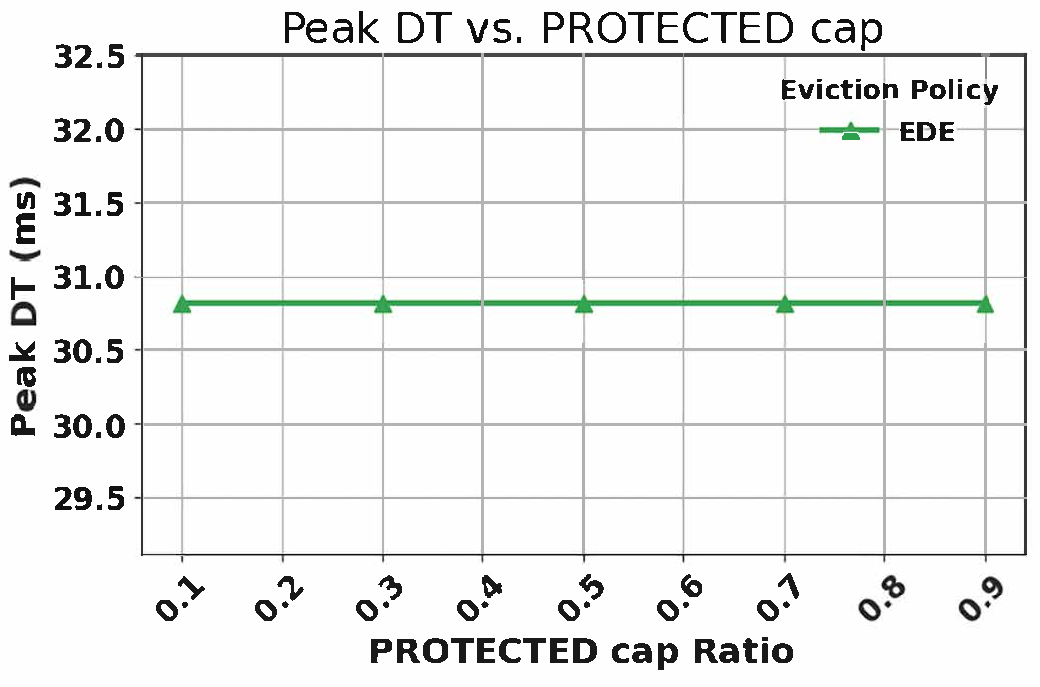
\includegraphics[width=0.50\textwidth]{a5_diagrams/A5_figure_3.png}
    \caption{: Peak DT vs. Protected Cap (EDE).} %The parameter is varied between 0.1 and 0.9 with an increment of 0.2. Results show minimal variation in Peak DT across the tested range, implying that the EDE policy maintains consistent service time regardless of segment allocation.}
    \label{fig:3}
\end{figure}



\begin{figure}[h]
%\begin{figure}[H]
    \centering
    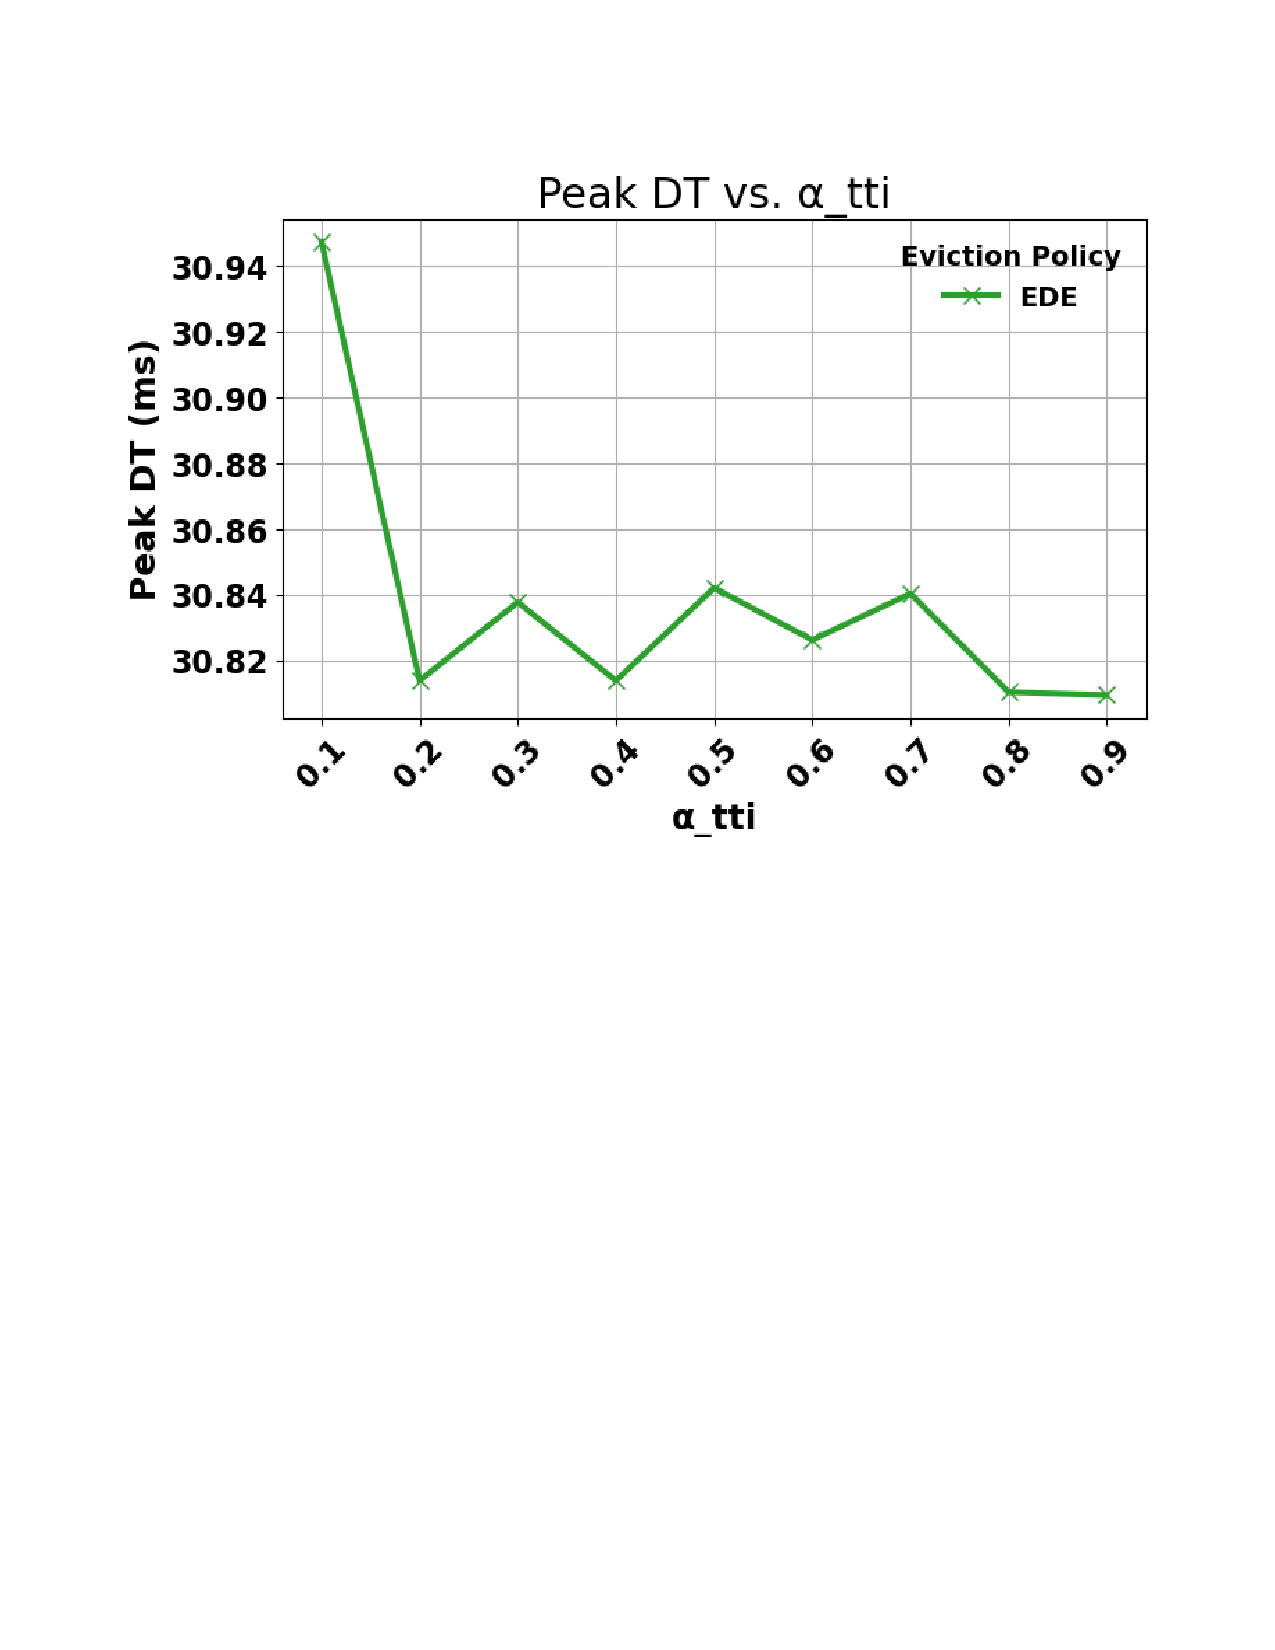
\includegraphics[width=0.50\textwidth]{a5_diagrams/A5_figure_4.pdf}
    \caption{: Peak DT vs $\alpha$tti (EDE).} % The parameter is varied between 0.1 and 0.9 with an increment of 0.1. Smaller values make the policy react faster to changes, while larger values make it more stable over time.}
    \label{fig:4}
\end{figure}

% support table
\begin{table}[h]
\centering
\caption{: Configuration and Metrics for EDE}
\label{tb:2}
\small
\begin{tabular}[t]{lp{5.2cm}}
\toprule
\textbf{Admission Policy} & Admit-All \\
\midrule
\textbf{Prefetch} & Disabled \\
\midrule
\textbf{Cache Size} & 366.475 GB \\
\midrule
\textbf{Trace Slices} & data/tectonic/201910/Region1/full\_0\_0.1.trace \\
\midrule
\textbf{Trace Sampling Ratio} & 0.1 \\
\midrule
\textbf{Write-rate Target} & 0 MB/s (target), 581.10 MB/s (actual) \\
\midrule
\textbf{Peak DT} & 29.1584 (P99.999 service time used) \\
\midrule
\textbf{Median DT} & 3.8891 (P50 service time used) \\
\midrule
\textbf{Hit Rate} & 0.0219 Hz (2.19\%) \\
\midrule
\textbf{Flash Write Rate} & 635.80 MB/s \\
\midrule
\textbf{RPOTECTED cap} & 0.1 $\sim$ 0.9 \\
\midrule
\textbf{$\alpha$tti} & 0.1 $\sim$ 0.9 \\
\bottomrule
\end{tabular}
\end{table}

% BEGINNING OF TABLE 4 

\begin{table*}[ht]
\centering
\caption{: Parameters Impact on Peak DT and Hit Rate. Summarizes the impact of individual parameters and policy settings on Peak DT and Hit Rate. It highlights how each tuning factor--ranging from $\tau_{\text{DT}}$ thresholds to $\alpha_{\text{tti}}$ smoothing--affects latency stability and cache efficiency. The results confirm that Baleen’s ML-guided approach achieves consistently lower Peak DT and higher hit rates compared to baseline eviction policies.}
\label{tab:dt_slru_trend_summary}
\begin{tabular}{p{3.2cm}p{6.5cm}p{6.5cm}}
\toprule
\textbf{Parameter} & \textbf{Peak DT} & \textbf{Hit Rate} \\
\midrule

\textbf{$\tau$DT} 
& Shows a U-shaped configuration. Very small $\tau$DT values (0.0002 to 0.001) admit various kinds of memory blocks without having an emphasis for reuse probability; this increases cache writes, and Peak DT. Mid-range settings (0.00141 to 0.01) keep Peak DT low by filtering out low admissions. Large values of DT (more than 0.01) lead to waste in flash space because not enough memory blocks are admitted to flash cache. 
& Highest in the mid range (0.01–0.02). Low $\tau$DT admits too many blocks and evicts blocks that have reuse potential prematurely. High $\tau$DT filters too and cause missed reuse. \\

\midrule

\textbf{PROTECTED Cap}
& Remains relatively stable across the full tested range. There is no strong improvement or degradation observed.
& Hit Rate slightly decreases by 0.5\% as the protected region grows from 0.5 to 0.9. A greater protection area reduces cache adaptability. This leads to diminishing returns in effective reuse. \\

\midrule

\textbf{$\alpha$tti}
& Peak DT improved slightly (by ~2–3\%) at lower $\alpha$tti values (0.01–0.1). However, as $\alpha$tti grew beyond 0.3, it began to delay evictions unnecessarily, resulting in a slight 1–2\% increase in Peak DT and reduced responsiveness.
& Declines with increasing $\alpha$tti because fewer reused blocks are kept long enough to contribute to hits. \\

\midrule

\textbf{Prefetching (Enabled vs. Disabled)} 
& Once prefetching is enabled, it tends to improve system stability, likely due to better I/O overlap.
& No noticeable increase in hit rate. \\

\midrule

\textbf{Policy Type (ML guided Baleen vs. Baselines)} 
& Baleen consistently shows lower Peak DT due to its implementation of ML-guided admission policy rather than heuristics
& Baleen achieves higher hit rates than DT SLRU and RejectX because it selectively admits blocks based on predicted future reuse probability rather than heuristics. \\

\bottomrule
\end{tabular}
\end{table*}



% END OF TABLE 4








\begin{figure}[ht!]
%\begin{figure}[H]
    \centering
    \includegraphics[width=0.50\textwidth]{a5_diagrams/A5_figure_5.pdf}
    \caption{: Normalized sensitivity comparison of Baleen parameters. Each curve shows Peak DT values normalized relative to each parameter’s minimum, with parameter ranges scaled to [0,1].}
    \label{fig:5}
\end{figure}

\begin{table}[t]
\centering
\caption{: Sensitivity Summary Across Ablated Parameters. Summarizes the observed sensitivity of each ablated parameter on Peak DT. The measured ranges show that all parameters cause only minor latency variation, confirming the overall stability of both DT-SLRU and EDE across their tested configurations.}
\label{tb:3}
\small
\begin{tabular}{lccp{2.8cm}}
\toprule
\textbf{Parameter} & \textbf{Policy} & \textbf{Range (ms)} & \textbf{Trend} \\
\midrule
$\tau$DT & DT-SLRU & 31.52--31.68 & Slight decrease at higher values \\
\midrule
PROTECTED cap & EDE & 30.81--30.81 & Stable (no visible effect) \\
\midrule
$\alpha$tti & EDE & 30.80--30.95 & Small fluctuations and mild sensitivity \\
\bottomrule
\end{tabular}
\end{table}


\clearpage
\section{Discussion}
% fill up entire 2 page
% no subsection in the report

\textbf{Figure 1 Analysis:}
Figure 1 shows that DT-Per-Byte Score (DT-SLRU), indeed has a huge impact on Peak DT, demonstrating a basic sensibility in terms of how hard the cache holds on to blocks. For very small DT-Per-Byte (e.g., 0.001), the cache still caches blocks that reduce the service time only a little. These blocks do not experience useful reuse before eviction so Peak DT does not offer improvement and flash writes increase since we maintain unneeded blocks. These blocks exist in flash cache without decreasing the backend load, thus resulting in waste of flash space and larger write amplification. 

As blocks are allowed admission without a clear demonstration of reused probability.
However, as the DT-Per-Byte Score moves upwards into the mid-range (on the order of 0.01 to 0.05), the cache starts retaining only blocks whose service time reduction gains are more pronounced. In this area, DT-SLRU filters out the low-utility blocks,  making Peak DT stabilize at a lower level than before with an overall service-time latency decrease. This is the optimum as far as Peak DT reduction is concerned. It is done, to let the flash cache be used efficiently, where blocks which are more likely to be reused (and thus more valuable in reducing access latency) can be admitted. The system strikes a balance between write endurance and performance boosts.
However, when the score exceeds that middle region (e.g., more than 0.05), the admission policy becomes less accommodating. There is a small number of blocks that cross the threshold for being kept in cache, so the flash storage capacity is left unused since not enough blocks are worthy to be kept in flash, preventing us from decreasing service time. This causes lost opportunities of caching high-impact blocks, and so the policy is less effective. 

%Therefore, Peak DT improvement saturates and no further advantage can be realized. This demonstrates that DT-SLRU is very sensitive to the choice of the DT-Per-Byte Score: thresholds with small values will waste flash for nothing, while too high threshold will not let the cache capture any clean reuse. Adjusting this parameter becomes particularly important in finding a trade-off between flash endurance and sustained service time benefits. Figure 1 clearly shows the need to choose DT scores corresponding to workload types and data reuse behaviors.










%This figure shows that the DT-Per-Byte Score parameter of DT-SLRU significantly affects Peak DT and reveals a fundamental trade-off between eviction aggressiveness and system efficiency. At low DT-Per-Byte Score thresholds (e.g., 0.001), the policy exhibits overly permissive eviction behavior where blocks are retained in cache despite minimal service-time savings potential, resulting in no visible Peak DT changes as items consume their limited reuse opportunities before eviction. However, this approach leads to excessive flash write operations, as memory blocks are speculatively preserved without strong evidence of sustained long-term utility, causing premature flash wear and inefficient cache utilization. In contrast, the policy's service-time-aware approach confronts this challenge by evaluating each item through the DT-per-byte scoring mechanism, a utility metric computed as service time saved divided by the number of bytes, enabling the system to determine which high-utility items justify their flash writes based on proven performance impact. Rather than using heuristic-based eviction decisions like LRU, DT-SLRU employs the academic testbed service time formula that accounts for both I/O operations at 11.5ms per operation and chunk transfers based on 143 MB/s disk bandwidth. The analysis demonstrates that DT-SLRU performance becomes suboptimal when thresholds are poorly tuned, emphasizing the waste of evicting blocks without evaluating their actual service-time savings potential.
This observation supports the principle that optimization for system-level metrics like service time is more robust than fine-tuning for hit rate alone, particularly in flash write rate-constrained environments where staying within endurance limits is crucial. As the DT-Per-Byte score increases toward middle range values (e.g., 0.01-0.05), the DT-SLRU policy becomes increasingly strict with respect to block eviction, tightening the eviction process to only evict blocks with a lower certainty of reuse before flash preservation. Only blocks demonstrating significant service time savings potential are kept in cache, resulting in more efficient cache operation with fewer, more stable rewrite operations. This sweet spot reflects the policy's focus on making admission decisions based on DT-per-byte scores to avoid evicting items with optimal utility-to-cost ratios. However, asthe DT-Per-Byte Score grows higher than this optimal range (e.g., >0.05), a critical issue emerges: too few blocks meet the threshold for retention, leading to flash capacity underutilization where frequently accessed blocks are sometimes evicted before reuse, causing Peak DT's decreasing trend plateaus. Unlike learned policies that generalize across various back-end workloads, DT-SLRU's static threshold approach plateaus at suboptimal performance levels, achieving only modest improvements.%


%\subsection{Figure 2: Hit Rate vs. DT(DT-SLRU Ablation)}
\textbf{Figure 2 Analysis:} Figure 2 illustrates that the DT-Per-Byte Score parameter of DT-SLRU significantly affects the cache Hit Rate and there is a trade-off among admitting recently accessed blocks and protecting flash write budget. At low DT-Per-Byte Score (e.g., 0.001), blocks are being kept in cache despite little reuse, and as a consequence block never used up all of its reuse opportunities and its hit rate is temporarily increased. However, this approach leads to a high amount of write operations in flash cache as memory blocks are evicted speculatively without strong evidence that their use is sustained long-term. 
By contrast, Baleen confronts this challenge by scoring each episode with the DT-per-byte score--a utility metric that is computed as DT saved divided by the number of bytes written at admission. This score enables the system to decide which high-utility episodes are admitted based on whether their flash writes can be justified. Rather than using heuristic based admission decisions like hit rates, Baleen learns access decisions from an offline OPT oracle which simulates the optimal caching behavior over the entire trace. The ML entrance rule then learns from this optimal label, so as to balance the endurance limit and reduce peak load \cite{wong2024baleen}.
The analysis in A4 shows that DT-SLRU performances were suboptimal even in terms of median DT compared to both baleen and RejectX, emphasizing the waste of admitting blocks without any discrimination on their DT savings. This observation supports the main point of the Baleen paper: optimization for system-end metrics like DT is more robust than fine tuning for hit rate only, particularly in flash write-rate constrained situations where it is crucial for flash caches need to stay strictly within their endurance limits.
As DT-Per-Byte Score is further increased toward middle range values (e.g., 0.01–0.05), the DT-SLRU policy becomes increasingly strict when it comes to letting blocks into flash and tightens up the admission process, only accepting with higher certainty that a block reuses before it can be preserved in flash. Only blocks that are highly reused can be written to flash. The result is that the cache is more efficient and rewrites tend to be fewer, more stable.  Unlike fixed thresholds, Baleen’s learned policy picks blocks predicted to provide long term gains to DT metrics without causing unnecessary flash wear.

Yet DT-Per-Byte Score grows higher than this optimal range (e.g., >0.05), an issue appears: here are too few blocks that meet the threshold and would be included for retention, underusing flash capacity. Often used blocks will sometimes be evicted before being reused, losing in hit rate. The hit rate curve in Figure 2 thus shows a peak in the middle range and falls off when higher thresholds are selected.
In contrast, ML-guided admission policy of Baleen learns DT-per-byte scores from an offline OPT oracle and uses the episodes to train a model that generalizes better across various kinds of backend workload. As seen from A4, Baleen achieves a much higher hit rate (approx. 9.3 percent) than all non-ML baselines and obtains better performance than DT-SLRU (and EDE), which only plateaued at about 3 percent.


%\subsection{Figure 3: Peak DT vs PROTECTED cap (EDE)}
\textbf{Figure 3 Analysis:} The figure illustrates how varying the PROTECTED cap parameter affects the Peak DT under the EDE policy. Five configurations were evaluated--0.1, 0.3, 0.5, 0.7, and 0.9--to satisfy the 0.2-increment requirement. Across the entire range, Peak DT remains nearly constant (around 31 ms), showing that the ratio between the protected and probationary cache segments has minimal effect on overall latency for this workload.

This stability suggests that under moderate data-reuse patterns, the system rarely benefits from dynamically changing the protected region. In such traces, object access intervals are already well-aligned with their episode deadlines, so the additional protection of frequently reused blocks does not significantly alter eviction decisions.
A smaller protected cap theoretically increases turnover, allowing faster adaptation to changing workloads; conversely, a larger cap favors long-term reuse by retaining popular blocks. However, in this experiment both effects appear balanced--neither more frequent refreshes nor longer retention significantly impacts peak latency.

This behavior matches the earlier A4 holistic evaluation, where EDE also demonstrated latency stability across parameter sweeps. The consistency across independent experiments confirms that EDE’s episode-deadline logic dominates its eviction decisions, effectively masking the influence of secondary configuration knobs such as the protected cap. This result reinforces EDE’s reliability in environments with medium reuse and stable I/O rates: performance remains predictable even when the cache allocation ratio is substantially varied.


%\subsection{Figure 4}
\textbf{Figure 4 Analysis:} Figure~\ref{fig:4} shows how the smoothing factor $\alpha_{\text{tti}}$ affects Peak DT under the EDE policy. This parameter controls how strongly the policy weighs the estimated time-to-idle (TTI) against the episode deadline when predicting which items to evict. At lower $\alpha_{\text{tti}}$ values (e.g., 0.1--0.2), the predictor reacts quickly to each new access, causing short-term volatility in eviction choices. These frequent shifts lead to a higher variance in service time and slightly elevated Peak DT values.

As $\alpha_{\text{tti}}$ increases, predictions become smoother: transient spikes in access time are averaged out, yielding more stable deadlines and gradually reducing Peak DT. Beyond 0.5, the curve flattens, implying that further smoothing no longer changes behavior meaningfully--the predictor’s responsiveness reaches equilibrium between agility and stability.

The results indicate that $\alpha_{\text{tti}}$ is more influential than the PROTECTED cap because it directly affects how the policy perceives temporal locality. Adjusting $\alpha_{\text{tti}}$ tunes the balance between responsiveness and steadiness, allowing the system to adapt to different workload dynamics. While overly small $\alpha_{\text{tti}}$ values make the cache react to noise, overly large ones delay adaptation to genuine phase changes. The narrow Peak DT range (approximately 30.8 – 30.9 ms) demonstrates that although EDE is generally stable, careful tuning of $\alpha_{\text{tti}}$ can slightly improve tail-latency control for bursty access traces.

This sensitivity also highlights that $\alpha_{\text{tti}}$ influences not only short-term latency but the long-term steadiness of eviction behavior. Moderate values (around 0.5–0.7) provide the best compromise, allowing the cache to stay responsive to phase changes while avoiding unnecessary churn. Under highly dynamic traces, this tuning prevents abrupt spikes in backend reads and helps maintain predictable service times. The parameter thus acts as a stabilizer within EDE’s feedback loop, ensuring smooth transitions between workload regimes. In practice, even small adjustments to $\alpha_{\text{tti}}$ can help sustain consistent disk-head utilization over extended runs, making this factor important for achieving durable and repeatable performance trends. Overall, this behavior confirms that EDE’s adaptability is driven more by temporal smoothing than by structural cache division, highlighting $\alpha_{\text{tti}}$ as a practical tuning knob for maintaining system resilience under changing conditions.

This aligns with the design intuition from the Baleen artifact: predictive smoothing enhances eviction precision by filtering out transient demand fluctuations, leading to steadier disk-head utilization. Thus, even within narrow numeric margins, $\alpha_{\text{tti}}$ remains a meaningful control lever for fine-grained tuning of EDE’s performance consistency.

%\subsection{Figure 5}

\textbf{Figure 5 Analysis:} This figure presents the normalized Peak DT values for all ablated parameters ($\tau_{\text{DT}}$ (DT-SLRU), PROTECTED cap (EDE), and $\alpha_{\text{tti}}$ (EDE)) summarizing how internal configuration knobs affect overall system sensitivity. Each curve depicts the relative deviation of Peak DT as the corresponding parameter is scaled to a normalized range of [0,1], enabling a direct visual comparison of the three sensitivity profiles.

For DT-SLRU, the $\tau_{\text{DT}}$ curve exhibits a mild downward slope, indicating that promotion-threshold adjustments have only a limited effect on Peak DT once the cache reaches a steady equilibrium of admissions and evictions. This behavior reflects DT-SLRU’s intrinsic DT awareness: its scoring mechanism already evaluates items based on service-time benefit rather than pure reuse frequency, allowing it to remain stable even as the promotion threshold changes by orders of magnitude. In essence, tuning $\tau_{\text{DT}}$ primarily shifts internal boundary conditions without altering the policy’s underlying decision logic.

The EDE parameters demonstrate even greater stability. The PROTECTED cap line remains nearly flat across the tested range (0.1–-0.9), confirming that varying the balance between protected and probationary regions exerts little impact under medium-reuse workloads. This outcome suggests that, within Baleen’s episode-deadline framework, eviction decisions are dominated by deadline proximity rather than by segment allocation. In contrast, the $\alpha_{\text{tti}}$ smoothing factor produces minor oscillations: when $\alpha_{\text{tti}}$ is too small, the predictor becomes overly reactive, causing transient spikes in Peak DT as it overfits to short bursts of activity. Conversely, when $\alpha_{\text{tti}}$ is too large, prediction updates become sluggish, underreacting to genuine workload phase shifts. These opposing tendencies yield small fluctuations ($\approx$ 0.15 ms range) without introducing systematic degradation, demonstrating that EDE can maintain tail-latency stability across both reactive and conservative configurations.

Supporting data from Tables 1-2 reinforce these graphical trends. Table~\ref{tb:1} summarizes the DT-SLRU configuration, where $\tau_{\text{DT}}$ sweeps between 0.0002 and 0.01 produced only 0.16 ms variation in Peak DT (31.52–31.68 ms). Table~\ref{tb:2} reports EDE’s parameter results, showing nearly identical performance across PROTECTED cap and $\alpha_{\text{tti}}$ experiments, with Peak DT values confined between 30.8 and 30.95 ms. Finally, Table~\ref{tb:3} aggregates these ranges in a unified sensitivity summary, confirming quantitatively that all ablated parameters contribute less than 1\% variation in Peak DT. This numerical stability provides concrete evidence that Baleen’s eviction logic, built around DT cost modeling, remains robust to parameter perturbations.

Overall, the combined sensitivity summary highlights that the three design parameters exert minimal influence on tail latency within the tested domain. Instead, the dominant performance factor lies in Baleen’s coordination between admission and prefetching, which continuously adapts to backend I/O dynamics. This finding generalizes the key insight of the Baleen paper: optimizing for DT yields consistent, low-variance performance even when internal thresholds shift substantially. In practice, this robustness implies that Baleen can be deployed with coarse-grained tuning--administrators need not finely calibrate every knob to achieve near-optimal latency--making it both operationally resilient and predictable under diverse workload conditions.




\clearpage
\section{Limitations}
% fill up haft page
The inherent difficulty of complete parameter exploration is one of the major challenges when empirically evaluating complex systems like the eviction policies under analysis. While ablation studies are an important methodology for isolating key design components to determine which factors contribute most to performance, this methodology has the underlying model assumption that parameters act independently. Pragmatic choices about the granularity of parameters and testing ranges have to be made by which, as it is pointed out in the limitations of this study, might potentially miss the true optimal configuration that lies between the coarsely grained steps, or not be able to capture the full curve by testing in too narrow a range. This ablation study gives proper insights into individual parameters, but has a number of constraints which could be taken as parameter granularity, range, and underlying model assumptions.

\textbf {Parameter Granularity:} It is important limitation in EDE policy. In Figure~\ref{fig:3} protected cap is varied in large 0.2 increments and this results in a completely flat line for Peak DT. This large step size means that it is impossible to determine whether there is actually no effect of the parameter, or whether there is an optimal, non-linear trend between the tested points. The 0.1 increments used in Figure~\ref{fig:4} demonstrate a very volatile pattern, indicating that even smaller steps would be required to portray the sensitivity of the parameter accurately. In Figure~\ref{fig:1} it was assumed that DT-per-byte-score and peak DT are independent of other parameters, a change in parameter other than these two can change the graph entirely.

\textbf{Dataset Representation:} In terms of data representation limited range of data was used due to which in analysis of DT-SLRU Figure~\ref{fig:1} and Figure~\ref{fig:2} have range from 0.000 to 0.010 which is not good enough as Peak DT in Figure~\ref{fig:1} is in downward trend and Hit rate in Figure~\ref{fig:2} is in upward trend which doesn't reflect the full range of the parameter and the optimum point where Peak DT may be at its lowest or Hit Rate at its highest. In Figure~\ref{fig:2} Hit Rate is data dependent the trend showing could be of a specific workload. If a workload or dataset is changed trend in graph may be different. In case of Figure~\ref{fig:4} $\alpha_{tti}$ is directly proportional to the dataset. Point where it looked instable and stable are not proper, it shows how well EDE is predicted over trace data. 

\textbf{Model Assumption:} The assumption model where the one parameter needs to be variable making all other constant which is a kind of limitation as it cannot provide good parameter interaction.
Taking in consideration in Figure~\ref{fig:3} flat nature of the graph Peak DT over protected cap ratio might not be true for specific value of $\alpha_{tti}$. Different protected cap ratio can interact differently and completely change the plot trend which can make different $\alpha_{tti}$ as an optimal value. For Figure~\ref{fig:5} cache and all hardware configuration similar for combined comparison for all policies while it may differ while working in different heterogeneous resource which could result in different results.



\clearpage
\section{Member Contributions}

\subsection{Anna Gorislavets}

\begin{itemize}
    \item Wrote Figure 5 Analysis, figures, and tables captions. Created Figure 5 and Table 4.
    \item Made the final formatting in the LaTeX.
    \item Used Overleaf and GitHub for collaboration, Jupyter Notebook for the code.
    \item Ensured quality by cross-checking the information, aligning with the rubric requirements.
    \item Participated in the final reading.
\end{itemize}

\subsection{Bikash Shyangtang}

\begin{itemize}
    \item Responsible for drafting limitation section.
    \item Analyzing different figures and help in running test in Jupyter Notebook.
    \item Use Overleaf for editing LaTeX and collaboration in Github.
    \item Ensured quality by comparing content with source papers and validating technical clarity with peers.
    \item Supported in integration of figures into LaTeX and helped organize group editing sessions.
\end{itemize}

\subsection{Hao Chen}

\begin{itemize}
    \item Run performance tests based on different BCacheSim configurations, data analysis, and plotting figures on JupyterLab.
    \item Create and format LaTeX templates and required figures.
    \item Github for version control, collaborative documentation, Overleaf for collaborative editing, JupyterLab for data analysis, and Notion for project management and task tracking.
    \item Quality was ensured by reviewing the checklist from the grading rubric and proofreading the entire paper with everyone present at the Teams Meeting before submission.
    \item Coordinated paper submission, Git commits, used Notion to manage assignment progress and deadline, set up routine Zoom/Teams meetups.
\end{itemize}

\subsection{Maoting Li}

\begin{itemize}
    \item Runned the tests for 5 values needed for Figure 2.
    \item Drafted 500+ words for the analysis of Figure 2 and helped to implement two support tables.
    \item Tools Used: Overleaf, Terminal.
    \item Verify the correctness of the first three figures based on gathered raw data.
    \item Contributed to overall editing by reviewing group sections for consistency in writing style and formatting.
\end{itemize}

\subsection{Salinrat Thanathapsakun}

\begin{itemize}
    \item Responsible for Figure 3 and its analysis.
    \item Interpreted experiment outputs, helped with the table captions.
    \item Used Overleaf for LaTeX formatting and collaboration; reviewed outputs for figure interpretation; Jupyter Notebook for coding.
    \item Verified that figure values and captions aligned with raw data logs and confirmed consistency between figures and text discussion.
    \item Coordinated integration of figures into the final Overleaf document and ensured consistent formatting according to style guidelines.
\end{itemize}
\begin{comment}
\section{Citations and Bibliographies}

The use of \BibTeX\ for the preparation and formatting of one's
references is strongly recommended. Authors' names should be complete
--- use full first names (``Donald E. Knuth'') not initials
(``D. E. Knuth'') --- and the salient identifying features of a
reference should be included: title, year, volume, number, pages,
article DOI, etc.

The bibliography is included in your source document with these two
commands, placed just before the \verb|\end{document}| command:
\begin{verbatim}
  \bibliographystyle{ACM-Reference-Format}
  \bibliography{bibfile}
\end{verbatim}
where ``\verb|bibfile|'' is the name, without the ``\verb|.bib|''
suffix, of the \BibTeX\ file.

Citations and references are numbered by default. A small number of
ACM publications have citations and references formatted in the
``author year'' style; for these exceptions, please include this
command in the {\bfseries preamble} (before the command
``\verb|\begin{document}|'') of your \LaTeX\ source:
\begin{verbatim}
  \citestyle{acmauthoryear}
\end{verbatim}


  Some examples.  A paginated journal article \cite{Abril07}, an
  enumerated journal article \cite{Cohen07}, a reference to an entire
  issue \cite{JCohen96}, a monograph (whole book) \cite{Kosiur01}, a
  monograph/whole book in a series (see 2a in spec. document)
  \cite{Harel79}, a divisible-book such as an anthology or compilation
  \cite{Editor00} followed by the same example, however we only output
  the series if the volume number is given \cite{Editor00a} (so
  Editor00a's series should NOT be present since it has no vol. no.),
  a chapter in a divisible book \cite{Spector90}, a chapter in a
  divisible book in a series \cite{Douglass98}, a multi-volume work as
  book \cite{Knuth97}, a couple of articles in a proceedings (of a
  conference, symposium, workshop for example) (paginated proceedings
  article) \cite{Andler79, Hagerup1993}, a proceedings article with
  all possible elements \cite{Smith10}, an example of an enumerated
  proceedings article \cite{VanGundy07}, an informally published work
  \cite{Harel78}, a couple of preprints \cite{Bornmann2019,
    AnzarootPBM14}, a doctoral dissertation \cite{Clarkson85}, a
  master's thesis: \cite{anisi03}, an online document / world wide web
  resource \cite{Thornburg01, Ablamowicz07, Poker06}, a video game
  (Case 1) \cite{Obama08} and (Case 2) \cite{Novak03} and \cite{Lee05}
  and (Case 3) a patent \cite{JoeScientist001}, work accepted for
  publication \cite{rous08}, 'YYYYb'-test for prolific author
  \cite{SaeediMEJ10} and \cite{SaeediJETC10}. Other cites might
  contain 'duplicate' DOI and URLs (some SIAM articles)
  \cite{Kirschmer:2010:AEI:1958016.1958018}. Boris / Barbara Beeton:
  multi-volume works as books \cite{MR781536} and \cite{MR781537}. A
  presentation~\cite{Reiser2014}. An article under
  review~\cite{Baggett2025}. A
  couple of citations with DOIs:
  \cite{2004:ITE:1009386.1010128,Kirschmer:2010:AEI:1958016.1958018}. Online
  citations: \cite{TUGInstmem, Thornburg01, CTANacmart}.
  Artifacts: \cite{R} and \cite{UMassCitations}.


\end{comment}
%
%% The next two lines define the bibliography style to be used, and
%% the bibliography file.
% \nocite{song2020lrb} % this will cite everything in *.bib file
%\citestyle{acmauthoryear}

\citestyle{acmnumeric}
\bibliographystyle{ACM-Reference-Format}
%\bibliographystyle{IEEEtran}
\clearpage
% \onecolumn make the document one column
\bibliography{ref}
%\bibliography{sample-base}

\clearpage

%%
%% If your work has an appendix, this is the place to put it.
% \appendix

% \section{Supplemental Material}

% \begin{figure}[ht!]
%   \centering
%   \includesvg[width=0.40\textwidth]{a1_diagrams/CSCI6806_storage_stack.svg}
%   \caption{Storage Architecture Diagram}
%   \label{fig:2}
% \end{figure}

\end{document}
\endinput
%%
%% End of file `sample-sigconf.tex'.
